\documentclass[border=10pt]{standalone}

\usepackage{tikz}
\usepackage{tikzsymbols}
\usetikzlibrary{calc,patterns,shapes.geometric}

\def\centerarc[#1](#2)(#3:#4:#5){\draw[#1] ($(#2)+({#5*cos(#3)},{#5*sin(#3)})$) arc (#3:#4:#5);}

\begin{document}
	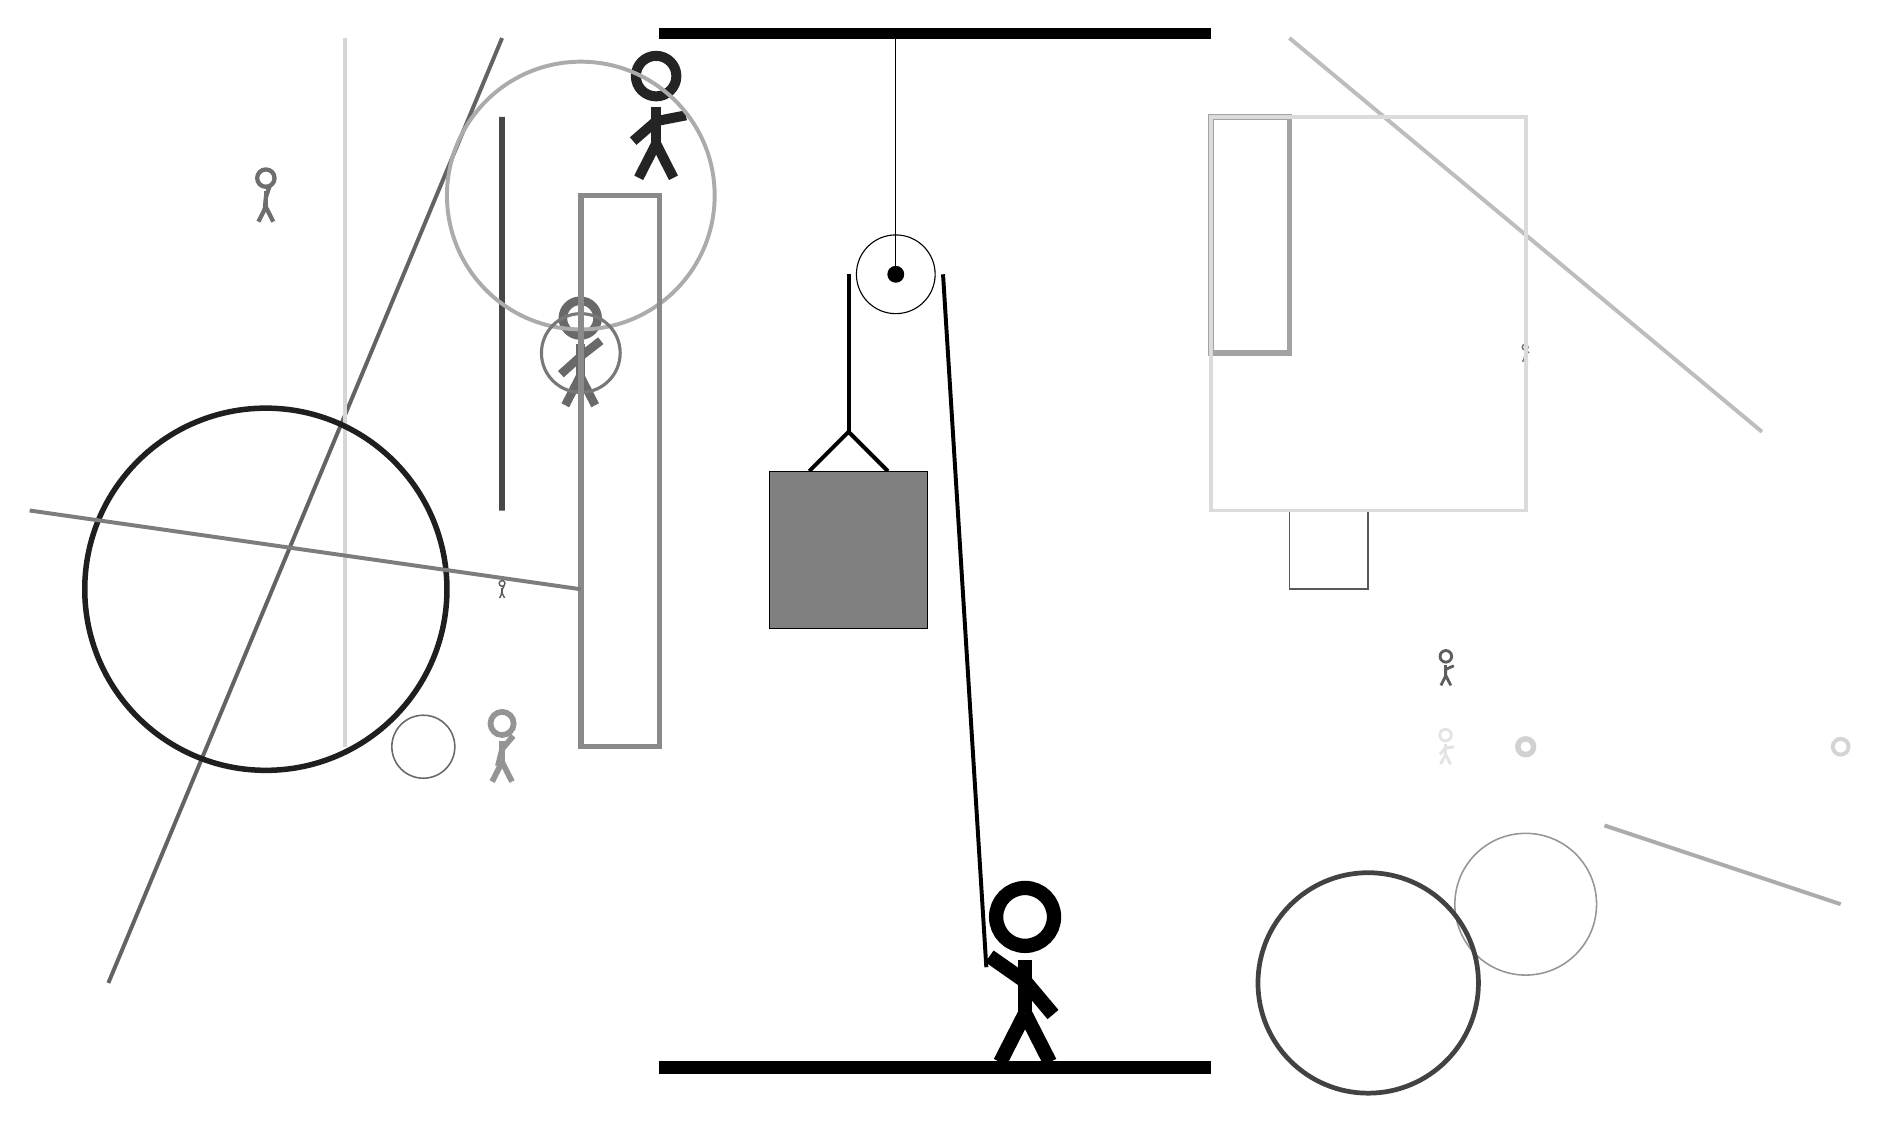
\begin{tikzpicture}
		%%%%% START %%%%%
		
		\draw[fill=black] (-2, 10) rectangle (5, 10.125);
		
		\draw (1, 7) circle (0.5);
		\draw[fill=black] (1, 7) circle (0.1);
		\draw (1, 10) -- (1, 7);
		
		\draw[line width=0.5mm] (-0.1, 4.5) -- (0.4, 5.0) -- (0.9, 4.5);
		\draw[fill=black!50] (-0.6, 4.5) rectangle (1.4, 2.5);
		
		\draw[line width=0.5mm] (0.4, 7) -- (0.4, 5.0);
		\centerarc[line width=0.5mm](1, 7)(0:180:0.6);
		\draw[line width=0.5mm](1.6, 7) -- (2.15, -1.8);
		
		\draw[line width=0.5mm, color=black!61](-4, 10) -- (-9, -2);
		
		\draw [line width=0.2mm, color=black!41](9, -1) circle (0.9);
		\node[line width=0.2mm, color=black!63] at (8, 2) {\Strichmaxerl[2][87][23]};
		\draw[line width=0.5mm, color=black!26](6, 10) -- (12, 5);
		\node[line width=0.3mm, color=black!42] at (-4, 1) {\Strichmaxerl[4][76][50]};
		\node[line width=0.2mm, color=black!56] at (9, 6) {\Strichmaxerl[1][78][22]};
		
		\draw[line width=0.7mm, color=black!36] (6, 9) rectangle (5, 6);
		\node[line width=0.6mm, color=black!11] at (8, 1) {\Strichmaxerl[2][48][7]};
		\draw[line width=0.5mm, color=black!33](10, 0) -- (13, -1);
		\node[line width=0.3mm, color=black!59] at (-3, 6) {\Strichmaxerl[6][42][38]};
		
		\draw [line width=0.2mm, color=black!59](-5, 1) circle (0.4);
		
		\draw[line width=0.2mm, color=black!65] (6, 3) rectangle (7, 4);
		\draw [line width=0.6mm, color=black!74](7, -2) circle (1.4);
		
		\draw[line width=0.5mm, color=black!16](-6, 10) -- (-6, 1);
		\draw[line width=0.7mm, color=black!72] (-4, 4) rectangle (-4, 9);
		\node[line width=0.3mm, color=black!64] at (-4, 3) {\Strichmaxerl[1][81][64]};
		
		\draw [line width=0.5mm, color=black!17](13, 1) circle (0.1);
		
		\draw [line width=0.7mm, color=black!88](-7, 3) circle (2.3);
		\draw [line width=0.7mm, color=black!18](9, 1) circle (0.1);
		\node[line width=0.5mm, color=black!86] at (-2, 9) {\Strichmaxerl[7][41][11]};
		\draw [line width=0.5mm, color=black!33](-3, 8) circle (1.7);
		
		\draw[line width=0.7mm, color=black!98] (6, -3) rectangle (6, -3);
		
		\draw[line width=0.5mm, color=black!14] (5, 9) rectangle (9, 4);
		\draw [line width=0.4mm, color=black!53](-3, 6) circle (0.5);
		\node[line width=0.4mm, color=black!57] at (-7, 8) {\Strichmaxerl[3][85][72]};
		
		\draw[line width=0.7mm, color=black!46] (-3, 1) rectangle (-2, 8);
		\draw[line width=0.5mm, color=black!51](-3, 3) -- (-10, 4);
		
		\node at (2.6, -1.9) {\Strichmaxerl[10][-35][-50]};
		
		\draw[fill=black] (-2, -3) rectangle (5, -3.15);
		
		%%%%% END %%%%%
	\end{tikzpicture}
\end{document}